\chapter{Methodology and Implementation}
\label{chap:methodology}

\section{Development Method}
I built the prototype in passes rather than from a frozen specification. The first pass was about naming the quality-workflow problem clearly. The second was a service-oriented sketch. After that came the user path, the agent path, and only then a hard look at what evidence would be needed to evaluate either. The proposal already asked for a phased evaluation: public and open-source material first, and only later, if approved, anonymized organizational artifacts. The mid-term presentation captured an earlier snapshot of the prototype and of that evaluation plan \cite{projectproposal,midtermpresentation}. This chapter describes the implementation. Comparative evaluation is still planned.

To write about the current state I went through the frontend, backend, agent service, tests, and deployment notes. Claims below are limited to paths I could actually find. The proposal and presentation explain what the project set out to do; they are not evidence that the planned experiments have been run.

\section{Requirements and Actors}
The main user is a quality engineer, a developer, or someone on a release call who needs structured testing guidance rather than another chat window. After signing in, that person supplies requirements or stories, optionally a diff or a test-run log, and then reads the response. A follow-up can reuse a session identifier. An administrator chooses the model provider and turns integrations on or off through environment settings.

\begin{table}[htbp]
\centering
\small
\begin{tabularx}{\textwidth}{p{0.22\textwidth}X}
\toprule
\textbf{Requirement} & \textbf{Prototype behavior} \\
\midrule
Context submission & Accepts requirements, user stories, code diffs, and optional session context through the authenticated assistance API. \\
Quality assistance & Returns a generated response that can include prioritized cases, test data, automation notes, and release risks. \\
Specialized analysis & Routes suitable requests to registered STLC agents for test design, execution-log analysis, change impact, defects, summaries, and readiness. \\
User separation & Associates assistance requests with the authenticated user and persists request inputs and responses in PostgreSQL. \\
Engineering context & Offers Jira Cloud story retrieval and GitHub pull-request or branch-diff retrieval when configured. \\
Operational configuration & Supports provider/model selection, containerized local startup, health checks, and production configuration checks. \\
\bottomrule
\end{tabularx}
\caption{Selected functional requirements and corresponding implemented behavior.}
\label{tab:functional-requirements}
\end{table}

\section{System Architecture}
The application has four main parts: the browser interface, the API, the database, and the agent runtime. The React and TypeScript frontend talks to the FastAPI backend. After access is checked, the backend stores the request, builds the agent message, and later stores the reply. A separate service runs the root agent and the specialists through Google ADK and a model abstraction. PostgreSQL holds users, requests, and integration records.

\begin{figure}[htbp]
\centering
\resizebox{0.98\textwidth}{!}{%
\begin{tikzpicture}[
  component/.style={draw,rounded corners,align=center,minimum width=3.0cm,minimum height=1.05cm,fill=gray!10},
  external/.style={draw,rounded corners,align=center,minimum width=2.7cm,minimum height=0.9cm,fill=blue!7},
  arrow/.style={-{Stealth[length=2.4mm]},thick}
]
\node[component] (browser) {User\\Browser};
\node[component,right=1.5cm of browser] (frontend) {React + TypeScript\\Web application};
\node[component,right=1.5cm of frontend] (backend) {FastAPI backend\\Auth, API, orchestration};
\node[component,below=1.3cm of backend] (db) {PostgreSQL\\Requests and connections};
\node[component,right=1.5cm of backend] (agent) {ADK agent service\\Root + STLC specialists};
\node[external,right=1.5cm of agent] (models) {Configured model\\Gemini / LiteLLM / Bedrock / Ollama};
\node[external,below=1.3cm of agent] (integrations) {Optional context\\Jira Cloud / GitHub};
\draw[arrow] (browser) -- (frontend);
\draw[arrow] (frontend) -- node[above,align=center]{HTTPS / REST\\JWT-authenticated} (backend);
\draw[arrow] (backend) -- (db);
\draw[arrow] (backend) -- node[above]{agent request} (agent);
\draw[arrow] (agent) -- (models);
\draw[arrow] (backend) -- (integrations);
\end{tikzpicture}}
\caption{Logical application architecture. Optional external integrations and model providers are enabled by configuration.}
\label{fig:system-architecture}
\end{figure}

Figure~\ref{fig:system-architecture} is the software that is actually in the repository. The AWS drawing that follows is a proposed target. It is not running today. The repository has deployment notes, but it does not provision that infrastructure.

\begin{figure}[H]
\centering
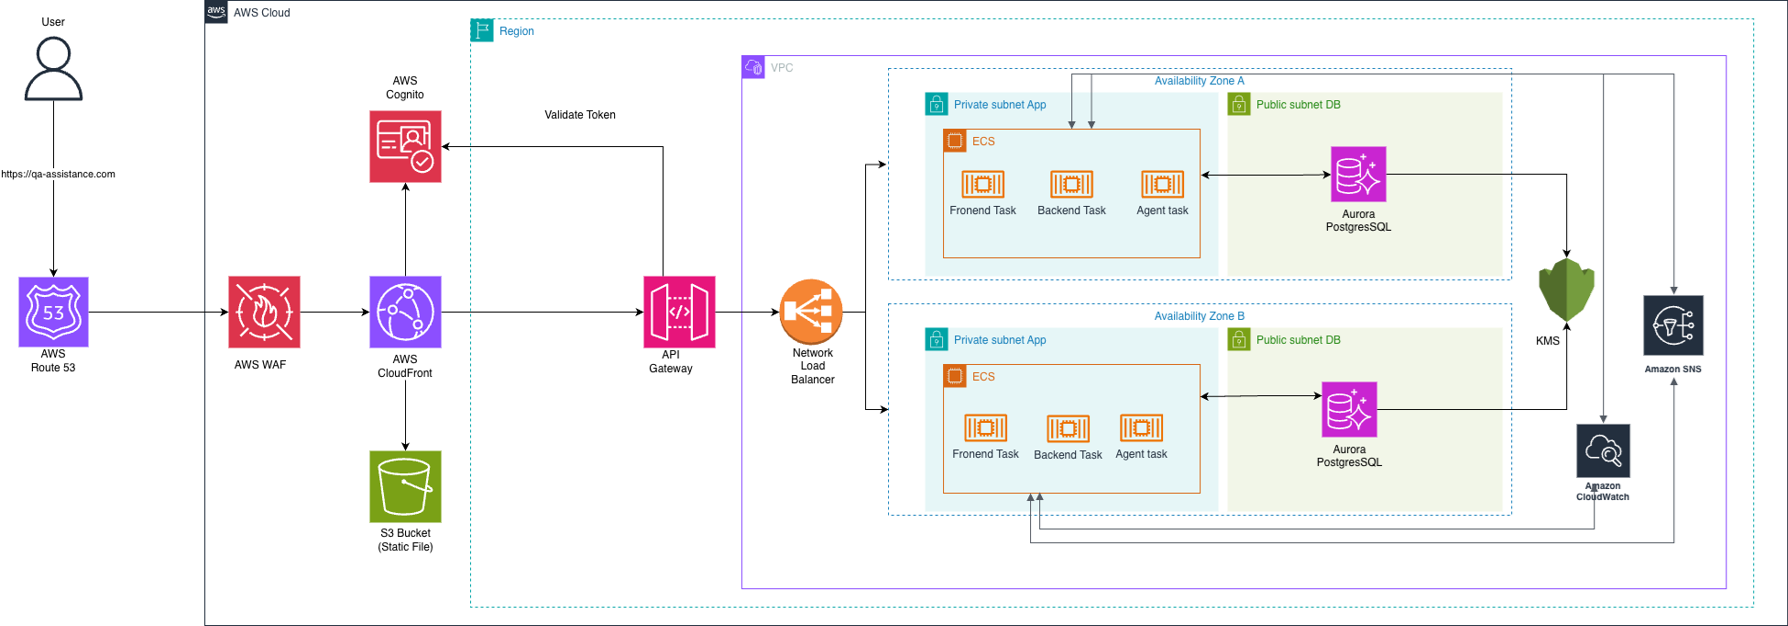
\includegraphics[width=0.98\textwidth,height=0.42\textheight,keepaspectratio]{SystemArchitecture.png}
\caption{Proposed AWS deployment architecture for the Quality Assistance application. This target design is not currently deployed by the repository.}
\label{fig:system-architecture-deployment}
\end{figure}

\subsection{Frontend}
The frontend covers sign-in, a dashboard for assistance requests, settings, and a short user guide. On the dashboard a user can type free-form requirements and stories, paste a code change, and start from sample requests: smoke planning, an end-to-end example, change impact, execution and reporting, automation, and a follow-up turn. If Jira is connected, assigned issues can fill the story field. If GitHub is connected, a pull-request or compare diff can be fetched rather than pasted. The reply is shown in the browser and can be downloaded as Markdown or HTML.

\subsection{Backend and Persistence}
The backend is a FastAPI service using asynchronous SQLAlchemy against PostgreSQL \cite{fastapidocs}. The \texttt{/api/assist} route is authenticated. It stores a request with its owner, source text, session identifier, status, timestamps, and, later, the response. It then builds a structured agent message and calls the agent service. Success and failure are both recorded. Errors go back to the frontend through the API's usual error path.

Users, assistance requests, Jira connections, and GitHub repository connections are stored as separate records. That is enough to look up an earlier submission. It is not enough to treat agent conversations as durable history. The current ADK runner keeps session state in memory, so a restart can drop a follow-up context that a user still has on screen.

\subsection{Agent Orchestration}
The root agent is named \texttt{quality\_assistance\_agent}. It is assembled with Google ADK, a configured model, logging callbacks, and the tools that are available at start-up \cite{googleadk}. For the supported cloud providers the root agent can hand work to registered sub-agents. The local Ollama path uses a single, consolidated instruction instead; the specialists are not transferred in that configuration. The backend prompt asks for prioritized test cases, suggested data, automation notes, and release risks, built from the requirements, stories, and diffs that were submitted.

\begin{table}[htbp]
\centering
\small
\begin{tabularx}{\textwidth}{p{0.06\textwidth}p{0.34\textwidth}X}
\toprule
\textbf{ID} & \textbf{Specialist} & \textbf{Implemented responsibility} \\
\midrule
S01 & Test case generation & Drafts structured, prioritized cases from requirements and stories, including positive, negative, and boundary scenarios. \\
S02 & Test data generation & Suggests representative and edge-case test data. \\
S03 & Test script automation & Suggests automation approaches and repeatable script outlines. \\
S04 & Test execution & Interprets supplied or simulated test-run results and highlights failures; it does not itself launch the user's test suite. \\
S05 & Self-healing test scripts & Recommends maintenance strategies when selectors or interfaces change; it does not directly edit repository files. \\
S06 & Change impact analysis & Relates supplied code diffs to potentially affected areas and regression scope. \\
S07 & Bug report generation & Structures failure information into an actionable defect report. \\
S08 & Test summary reporting & Summarizes test outcomes for stakeholders. \\
S09 & Release readiness evaluation & Weighs supplied test and risk signals and provides a reasoned recommendation. \\
\bottomrule
\end{tabularx}
\caption{Registered specialist agents and the scope described by their instructions.}
\label{tab:agents}
\end{table}

The router maps requirement and story text to the test-case and test-data agents, diffs to change-impact analysis, execution logs to the execution, defect, and summary agents, and release questions to readiness. There is also a requirement-summarization tool on the root agent. This is prompt-driven routing. There is no separate deterministic workflow engine sitting beside it.

\begin{figure}[H]
\centering
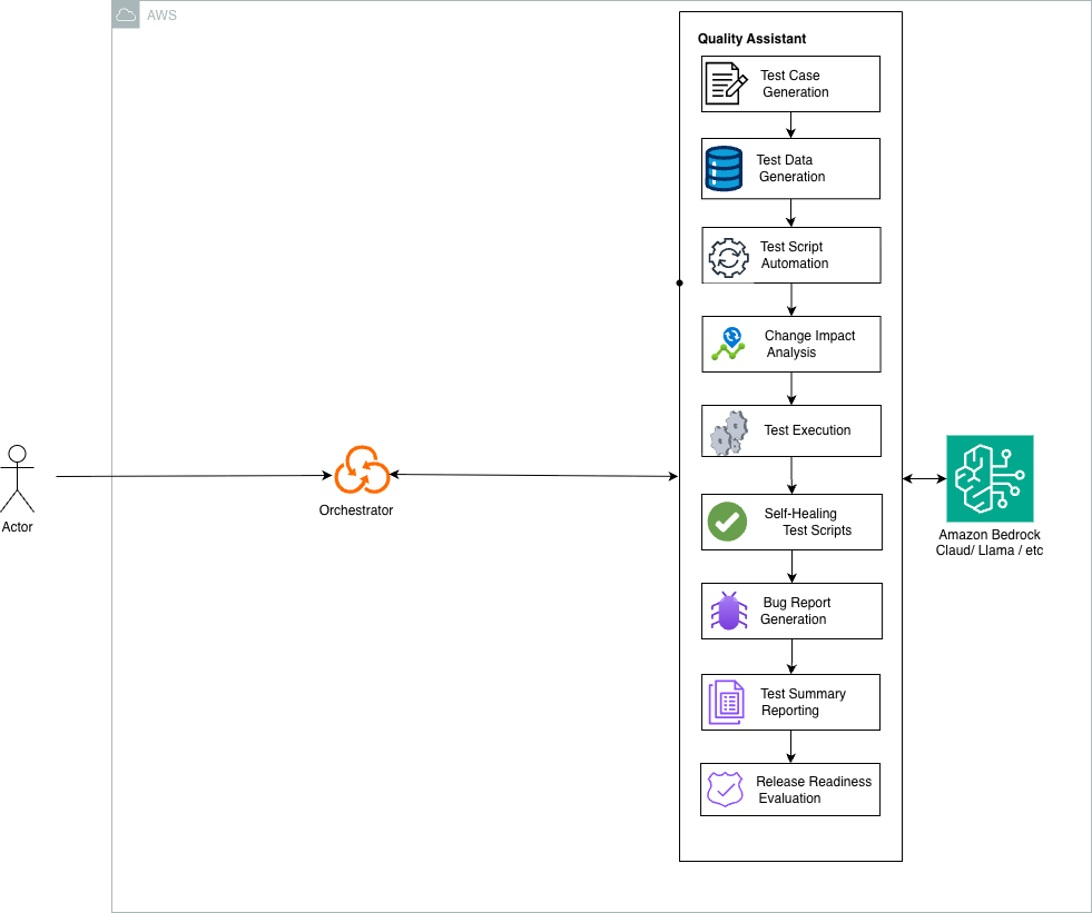
\includegraphics[width=0.72\textwidth,height=0.45\textheight,keepaspectratio]{agentic_flow.jpg}
\caption{Illustrative agentic workflow showing orchestration among the root agent and specialist agents.}
\label{fig:agentic-flow}
\end{figure}

\begin{algorithm}[htbp]
\caption{Assistance request processing}
\label{alg:assistance}
\begin{algorithmic}[1]
\Require Authenticated user $u$, requirements $r$, optional stories $s$, diff $d$, session $q$
\State Validate the request and associate it with $u$
\State Persist request inputs with status \texttt{processing}
\State Construct a message from $r$, $s$, and $d$
\State Resolve or create an agent session for $u$
\State Invoke the root agent with the message and session
\State Route to one or more specialists according to the request context
\State Collect the generated response from the agent events
\If{agent call succeeds}
  \State Persist session identifier, response, and status \texttt{completed}
\Else
  \State Persist failure status and return an explicit service error
\EndIf
\State Return the request identifier, session, response, and status
\end{algorithmic}
\end{algorithm}

\begin{figure}[H]
\centering
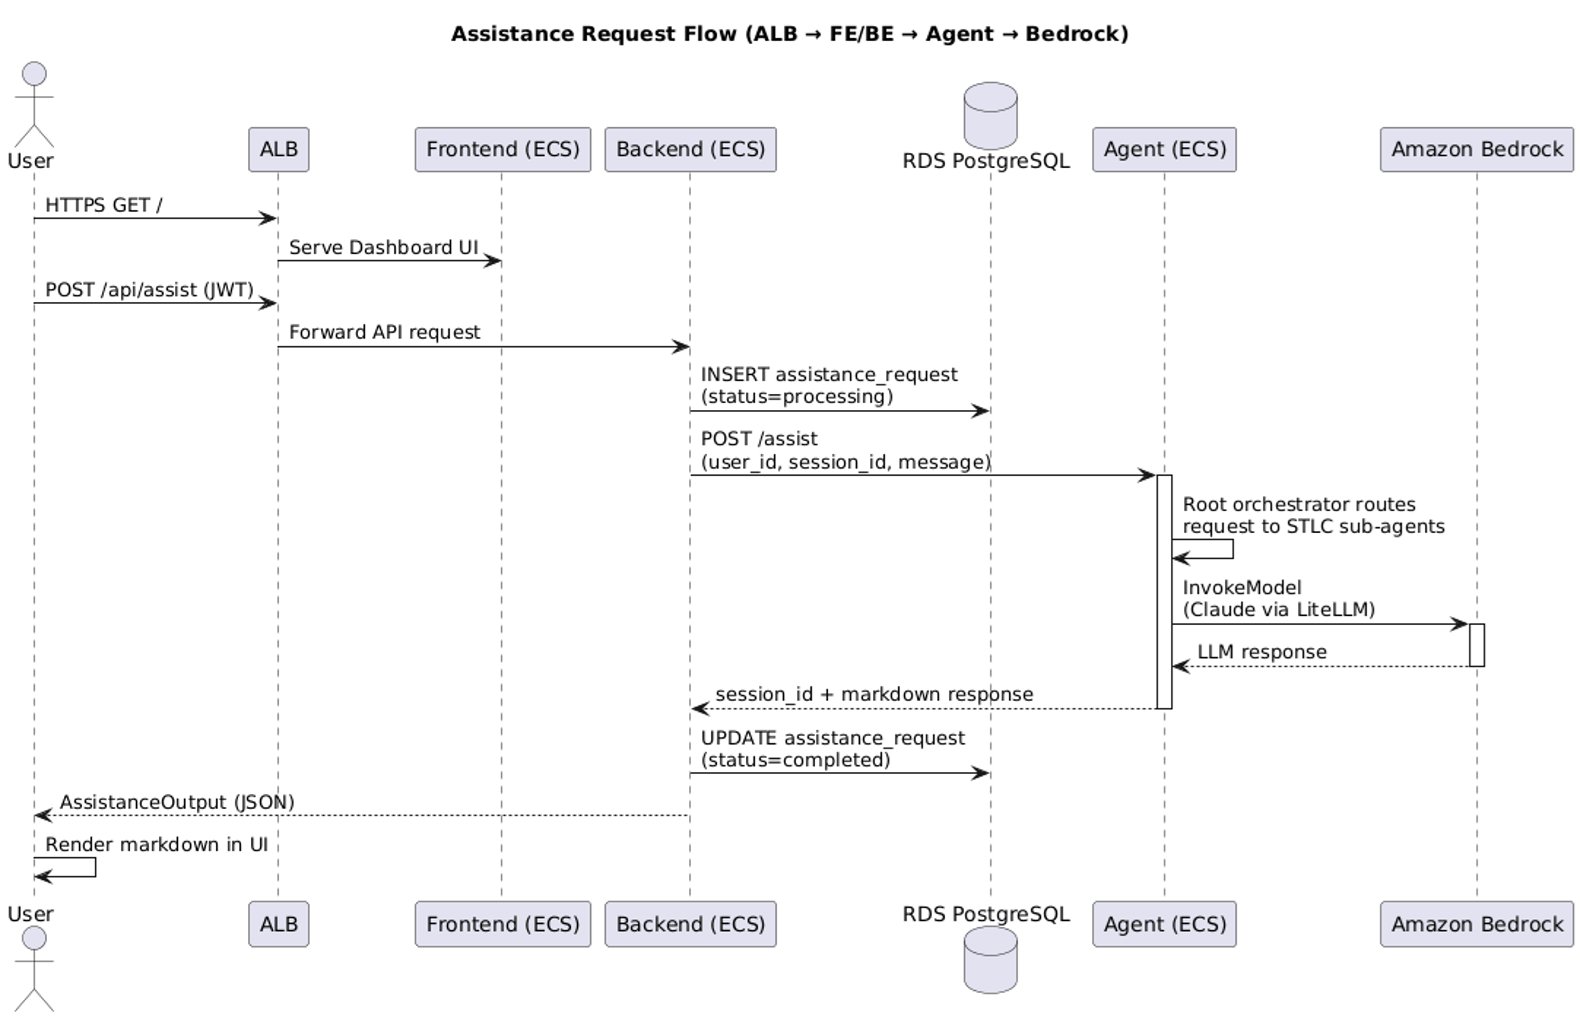
\includegraphics[width=0.92\textwidth,height=0.48\textheight,keepaspectratio]{sequence_daigram.png}
\caption{Illustrative request sequence through the application services for the deployment configuration shown.}
\label{fig:request-sequence}
\end{figure}

\subsection{External Integrations and Model Providers}
Jira Cloud uses OAuth 2.0, a short-lived state record, and Jira APIs to list a user's assigned issues and to fetch issue detail. GitHub settings store a repository and an encrypted personal access token; the backend can then pull a pull-request diff or compare two references. Microsoft Entra single sign-on is optional. The agent configuration accepts Gemini, LiteLLM, Amazon Bedrock, and Ollama, provided credentials and models are available. Those are options in the code. They are not a claim that every provider was benchmarked on the same tasks.

\section{Security and Data Handling}
Assistance records belong to the signed-in user. JWT access tokens are issued after registration or login. Password handling is delegated to the project's password manager. Jira and GitHub credentials are stored encrypted. Jira OAuth state is a digest and it expires. In production the settings check looks for real secrets, an encryption key, explicit HTTPS origins, database TLS, and non-default database credentials. The ECS guide describes a pattern with private application and database services, IAM roles, and managed secrets.

Requirements, stories, diffs, and test results can easily contain proprietary information. The application stores them with the request and sends them to whatever model provider is configured. Anyone deploying this has to pick a provider and retention policy that their organization will accept, restrict who can see stored data, rotate credentials, and keep secrets out of the prompt. The controls in the prototype reduce accidental exposure. They do not replace a privacy assessment, a threat model, an independent review, or an internal approval.

\section{Deployment and Operations}
For local work the repository has a Docker Compose stack covering PostgreSQL, frontend, backend, and agent. There are also scripts for a local frontend and Python services against a local or containerized database. The AWS ECS Fargate notes describe a pilot with separate containers, RDS PostgreSQL, an Application Load Balancer, and a chosen model provider. That document is a checklist. It is not infrastructure-as-code, and this report does not claim that an AWS production environment has been stood up.

\section{Quality Attributes}
\begin{itemize}
  \item \textbf{Modularity:} frontend, API, persistence, and agent service are separate processes; specialists are registered on their own.
  \item \textbf{Configurability:} model providers, endpoints, integrations, and production flags come from the environment.
  \item \textbf{Traceability:} the backend stores each user's inputs and responses; a formal requirement-to-case evidence trail and durable agent memory are still missing.
  \item \textbf{Availability:} health and readiness endpoints and container notes help operations; how resilient a real deployment is depends on the topology that is actually chosen.
  \item \textbf{Reliability:} the backend has explicit error paths and settings checks. Generated quality artifacts still need a person to read them, and they still need an empirical evaluation.
\end{itemize}
